% !TeX spellcheck = en_US
% !TeX encoding = UTF-8 

\documentclass[14pt,a4paper]{extarticle}

\usepackage[english]{babel}
\usepackage[utf8]{inputenc}
\usepackage{setspace} 
\usepackage[a4paper,
	left=30mm,
	right=10mm,
	top=20mm,
	bottom=20mm]{geometry}
\usepackage{amsmath,amssymb,amsthm}
\usepackage{cite}
\usepackage{graphicx} 
\usepackage{subfigure,subcaption}
\usepackage{kprjHSE} 
\usepackage{tikz}
\usepackage{xcolor,tabularray}
\usepackage{wrapfig}

\usetikzlibrary{positioning}

\renewcommand{\labelenumii}{\arabic{enumi}.\arabic{enumii}}

\lstset{
	frame=single,
	basicstyle=\ttfamily,
	breaklines=true,
	tabsize=4
}

\LabWork
\LabWorkNo{2}

\FirstAuthor{M.D.~Kirdin}
\FirstConsultant{A.~Tomat}
\SecondConsultant{M.~Zueva}
\discipline{Ordered Sets for Data Analysis}
\faculty{Faculty of Computer Science}
\chair{School of Data Analysis and Artificial Intelligence}
\chief{S.O.~Kuznetsov}
\workyear{2024}

\onehalfspacing

\begin{document}
	\maketitle
	
	\subsection*{Question 1}
	\noindent\textbf{Task.} Given the following formal context, find all formal concepts, draw the concept lattice and find all non-trivial implications.
	
	\begin{center}
		\begin{tblr}{
				width=\linewidth, 
				colspec={|X[c]|X[c]|X[c]|X[c]|X[c]|X[c]|}
				}
			\hline
			 & a & b & c & d & e\\
			\hline
			1 & 1 &  & 1 &  & 1\\
			\hline
			2 & 1 &  & 1 & 1 & \\
			\hline
			3 & 1 &  &  & 1 & 1\\
			\hline
			4 & 1 & 1 &  & 1 & \\
			\hline
			5 & 1 & 1 &  &  & 1\\
			\hline
		\end{tblr}
	\end{center}
	 
	\noindent\textbf{Solution.} Let the set of all objects be denoted as $G=\{1,\, 2,\, 3,\, 4,\, 5\}$ and the set of all attributes as $M=\{a,\, b,\, c,\, d,\, e\}$. We will condense all the data about formal concepts in this context into a table, where $A \subseteq M$ is \textit{extent} of a formal concept and $B\subseteq G$ is its \textit{intent}.
	 
	\begin{center}
		\begin{tblr}{
	 			width=\linewidth, 
	 			colspec={|X[c]|X[c]|X[c]|X[c]|}
	 		}
	 		\hline
	 		$A$ & $B=A^\prime$ & $A^{\prime\prime}$ & Formal concept?\\
	 		\hline
	 		$\{\emptyset_{M}\}$ & $G$ & $\{\emptyset_{M}\}$ & \SetCell{green9} Yes \\
	 		\hline
	 		$M$ & $\{a\}$ & $M$ & \SetCell{green9} Yes \\
	 		\hline
	 		$\{1\}$ & $\{a,\, c,\, e\}$ & $\{1\}$ & \SetCell{green9} Yes \\
	 		\hline
	 		$\{2\}$ & $\{a,\, c,\, d\}$ & $\{2\}$ & \SetCell{green9} Yes \\
	 		\hline
	 		$\{3\}$ & $\{a,\, d,\, e\}$ & $\{3\}$ & \SetCell{green9} Yes \\
	 		\hline
	 		$\{4\}$ & $\{a,\, b,\, d\}$ & $\{4\}$ & \SetCell{green9} Yes \\
	 		\hline
	 		$\{5\}$ & $\{a,\, b,\, e\}$ & $\{5\}$ & \SetCell{green9} Yes \\
	 		\hline
	 		$\{1,\, 2\}$ & $\{a,\, c\}$ & $\{1,\, 2\}$ & \SetCell{green9} Yes \\
	 		\hline
	 		$\{1,\, 3\}$ & $\{a\}$ & $M$ & No \\
	 		\hline
	 		$\{1,\, 4\}$ & $\{a\}$ & $M$ & No \\
	 		\hline
	 		$\{1,\, 5\}$ & $\{a,\, e\}$ & $\{1,\, 3,\, 5\}$ & No \\
	 		\hline
	 		$\{2,\, 3\}$ & $\{a,\, d\}$ & $\{2,\, 3,\, 4\}$ & No \\
	 		\hline
	 		$\{2,\, 4\}$ & $\{a,\, d\}$ & $\{2,\, 3,\, 4\}$ & No \\
	 		\hline
		\end{tblr}
		\begin{tblr}{
	 			width=\linewidth, 
	 			colspec={|X[c]|X[c]|X[c]|X[c]|}
	 		}
	 		\hline
	 		$A$ & $B=A^\prime$ & $A^{\prime\prime}$ & Formal concept?\\
	 		\hline
	 		$\{2,\, 5\}$ & $\{a\}$ & $M$ & No \\
	 		\hline
	 		$\{3,\, 4\}$ & $\{a,\, d\}$ & $\{2,\, 3,\, 4\}$ & No \\
	 		\hline
	 		$\{3,\, 5\}$ & $\{a\}$ & $M$ & No \\
	 		\hline
	 		$\{4,\, 5\}$ & $\{a,\, b\}$ & $\{4,\, 5\}$ & \SetCell{green9} Yes \\
	 		\hline
	 		$\{1,\, 2,\, 3\}$ & $\{a\}$ & $M$ & No\\
	 		\hline
	 		$\{1,\, 2,\, 4\}$ & $\{a\}$ & $M$ & No\\
	 		\hline
	 		$\{1,\, 2,\, 5\}$ & $\{a\}$ & $M$ & No\\
	 		\hline
	 		$\{1,\, 3,\, 4\}$ & $\{a\}$ & $M$ & No\\
	 		\hline
	 		$\{1,\, 3,\, 5\}$ & $\{a,\, e\}$ & $\{1,\, 3,\, 5\}$ & \SetCell{green9} Yes\\
	 		\hline
	 		$\{1,\, 4,\, 5\}$ & $\{a\}$ & $M$ & No\\
	 		\hline
	 		$\{2,\, 3,\, 4\}$ & $\{a,\, d\}$ & $\{2,\, 3,\, 4\}$ & \SetCell{green9} Yes\\
	 		\hline
	 		$\{2,\, 3,\, 5\}$ & $\{a\}$ & $M$ & No\\
	 		\hline
	 		$\{3,\, 4,\, 5\}$ & $\{a\}$ & $M$ & No\\
	 		\hline
	 		$\{1,\, 2,\, 3,\, 4\}$ & $\{a\}$ & $M$ & No\\
	 		\hline
	 		$\{1,\, 2,\, 3,\, 5\}$ & $\{a\}$ & $M$ & No\\
	 		\hline
	 		$\{1,\, 2,\, 4,\, 5\}$ & $\{a\}$ & $M$ & No\\
	 		\hline
	 		$\{1,\, 3,\, 4,\, 5\}$ & $\{a\}$ & $M$ & No\\
	 		\hline
	 		$\{2,\, 3,\, 4,\, 5\}$ & $\{a\}$ & $M$ & No\\
	 		\hline
		\end{tblr}
	\end{center}
	 
	Having found all the formal concepts, we are able to construct the concept lattice.
	 
	\begin{center}
	\resizebox{\linewidth}{10em}{%
		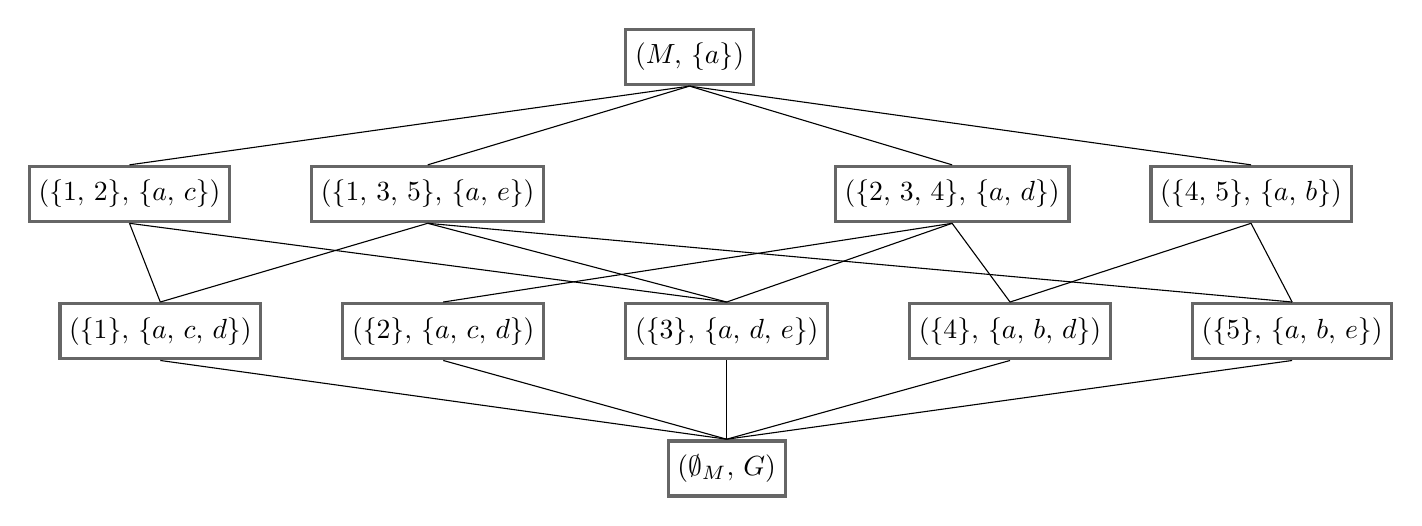
\begin{tikzpicture}[
	 	squarednode/.style={rectangle, draw=black!60, very thick, minimum size=7mm},
	 	]
	 	%Nodes
	 	\node[squarednode]      (toplayer)   {$(M,\, \{a\})$};
	 	\node[squarednode]      (3layer3)    [below right=of toplayer] {$(\{2,\, 3,\, 4\},\, \{a,\, d\})$};
	 	\node[squarednode]      (3layer4)    [right=of 3layer3] {$(\{4,\, 5\},\, \{a,\, b\})$};
	 	\node[squarednode]      (3layer2)    [below left=of toplayer] {$(\{1,\, 3,\, 5\},\, \{a,\, e\})$};
	 	\node[squarednode]      (3layer1)    [left=of 3layer2] {$(\{1,\, 2\},\, \{a,\, c\})$};
	 	\node[squarednode]      (2layer3)    [below right=of 3layer2] {$(\{3\},\, \{a,\, d,\, e\})$};
	 	\node[squarednode]      (2layer2)    [left=of 2layer3] {$(\{2\},\, \{a,\, c,\, d\})$};
	 	\node[squarednode]      (2layer4)    [right=of 2layer3] {$(\{4\},\, \{a,\, b,\, d\})$};
	 	\node[squarednode]      (2layer1)    [left=of 2layer2] {$(\{1\},\, \{a,\, c,\, d\})$};
	 	\node[squarednode]      (2layer5)    [right=of 2layer4] {$(\{5\},\, \{a,\, b,\, e\})$};
	 	\node[squarednode]      (bottomlayer)    [below=of 2layer3] {$(\emptyset_{M},\, G)$};
	 	
	 	%Lines
	 	\draw[-] (toplayer.south) -- (3layer4.north);
	 	\draw[-] (toplayer.south) -- (3layer3.north);
	 	\draw[-] (toplayer.south) -- (3layer2.north);
	 	\draw[-] (toplayer.south) -- (3layer1.north);
	 	\draw[-] (3layer1.south) -- (2layer1.north);
	 	\draw[-] (3layer1.south) -- (2layer3.north);
	 	\draw[-] (3layer2.south) -- (2layer1.north);
	 	\draw[-] (3layer2.south) -- (2layer3.north);
	 	\draw[-] (3layer2.south) -- (2layer5.north);
	 	\draw[-] (3layer3.south) -- (2layer2.north);
	 	\draw[-] (3layer3.south) -- (2layer3.north);
	 	\draw[-] (3layer3.south) -- (2layer4.north);
	 	\draw[-] (3layer4.south) -- (2layer4.north);
	 	\draw[-] (3layer4.south) -- (2layer5.north);
	 	\draw[-] (2layer1.south) -- (bottomlayer.north);
	 	\draw[-] (2layer2.south) -- (bottomlayer.north);
	 	\draw[-] (2layer3.south) -- (bottomlayer.north);
	 	\draw[-] (2layer4.south) -- (bottomlayer.north);
	 	\draw[-] (2layer5.south) -- (bottomlayer.north);
		\end{tikzpicture}
	}
	\end{center}
	 
	\begin{definition}
		$A \rightarrow B$, where $A, B \subseteq M$ holds in context $(G, M, I)$ if $A^{\prime}\subseteq B^{\prime}$, i.e., each object having all attributes from A also has all attributes from B.
	\end{definition}
	 
	Therefore, we can construct a table of all the subsets of $M$, which upon application of prime operator return nonempty sets to look for all non-trivial implications.
	
	\begin{center}
		\begin{tblr}{width=\linewidth, colspec={|X[c]|X[c]|X[c]|X[c]|X[c]|X[c]|}}
			\hline
			$A$ & $A^\prime$ & $A^{\prime\prime}\setminus A$ & $A$ & $A^\prime$ & $A^{\prime\prime}\setminus A$\\
			\hline
			$\{a\}$ & $G$ & $\emptyset_{M}$ & $\{a,\, b,\, d\}$ & $\{4\}$ & $\emptyset_{M}$\\
			\hline
			$\{b\}$ & $\{4,\, 5\}$ & $\{a\}$ & $\{a,\, b,\, e\}$ & $\{5\}$ & $\emptyset_{M}$\\
			\hline
			$\{c\}$ & $\{1,\, 2\}$ & $\{a\}$ & $\{a,\, c,\, d\}$ & $\{2\}$ & $\emptyset_{M}$\\
			\hline
			$\{d\}$ & $\{2,\, 3,\, 4\}$ & $\{a\}$ & $\{a,\, c,\, e\}$ & $\{1\}$ & $\emptyset_{M}$\\
			\hline
			$\{e\}$ & $\{1,\, 3,\, 5\}$ & $\{a\}$ & $\{a,\, d,\, e\}$ & $\{3\}$ & $\emptyset_{M}$\\
			\hline
			$\{a,\, b\}$ & $\{4,\, 5\}$ & $\emptyset_{M}$ & $\{b,\, c,\, d\}$ & $\emptyset_{G}$ & $\{a,\, e\}$\\
			\hline
			$\{a,\, c\}$ & $\{1,\, 2\}$ & $\emptyset_{M}$ & $\{b,\, c,\, e\}$ & $\emptyset_{G}$ & $\{a,\, d\}$\\
			\hline
			$\{a,\, d\}$ & $\{2,\, 3,\, 4\}$ & $\emptyset_{M}$ & $\{b,\, d,\, e\}$ & $\emptyset_{G}$ & $\{a,\, c\}$\\
			\hline
			$\{a,\, e\}$ & $\{1,\, 3,\, 5\}$ & $\emptyset_{M}$ & $\{c,\, d,\, e\}$ & $\emptyset_{G}$ & $\{a,\, b\}$\\
			\hline
			$\{b,\, c\}$ & $\emptyset_{G}$ & $\{a,\, d,\, e\}$ & $\{a,\, b,\, c,\, d\}$ & $\emptyset_{G}$ & $\{e\}$\\
			\hline
			$\{b,\, d\}$ & $\{4\}$ & $\{a\}$ & $\{a,\, b,\, c,\, e\}$ & $\emptyset_{G}$ & $\{d\}$\\
			\hline
			$\{b,\, e\}$ & $\{5\}$ & $\{a\}$ & $\{a,\, b,\, d,\, e\}$ & $\emptyset_{G}$ & $\{c\}$\\
			\hline
			$\{c,\, d\}$ & $\{2\}$ & $\{a\}$ & $\{a,\, c,\, d,\, e\}$ & $\emptyset_{G}$ & $\{b\}$\\
			\hline
			$\{c,\, e\}$ & $\{1\}$ & $\{a\}$ & $\{b,\, c,\, d,\, e\}$ & $\emptyset_{G}$ & $\{a\}$\\
			\hline
			$\{d,\, e\}$ & $\{3\}$ & $\{a\}$ & $\emptyset_M$ & G & Trivial\\
			\hline
			$\{a,\, b,\, c\}$ & $\emptyset_{G}$ & $\{d,\, e\}$ & & & \\
			\hline
		\end{tblr}
	\end{center}
	
	\noindent According to the table there are following non-trivial implications: $\{b\}\rightarrow \{a\}$, $\{c\}\rightarrow \{a\}$, $\{d\}\rightarrow \{a\}$, $\{e\}\rightarrow \{a\}$, $\{b,\, c\}\rightarrow\{a,\, d,\, e\}$, $\{a,\, b,\, c\}\rightarrow\{d,\, e\}$, $\{b,\, d\}\rightarrow \{a\}$, $\{b,\, e\}\rightarrow \{a\}$, $\{c,\, e\}\rightarrow \{a\}$, $\{c,\, d\}\rightarrow \{a\}$, $\{d,\, e\}\rightarrow \{a\}$, $\{b,\, c,\, d\}\rightarrow\{a,\, e\}$, $\{b,\, c,\, e\}\rightarrow\{a,\, d\}$, $\{b,\, d,\, e\}\rightarrow\{a,\, c\}$, $\{c,\, d,\, e\}\rightarrow\{a,\, b\}$, $\{a,\, b,\, c,\, d\}\rightarrow\{e\}$, $\{a,\, b,\, c,\, e\}\rightarrow\{d\}$, $\{a,\, b,\, d,\, e\}\rightarrow\{c\}$, $\{a,\, c,\, d,\, e\}\rightarrow\{b\}$, $\{b,\, c,\, d,\, e\}\rightarrow\{a\}$.
	\newpage
	 
	\subsection*{Question 2}
	 
	\noindent\textbf{Task.} Using the diagram find:
	\begin{enumerate}
		\item $f\land m,\, a\lor l,\, i\land k$;
		\item $a\land(c\lor d),\, (i\land g)\lor(c\land d),\, \bigvee(b,\, c,\, d)$;
		\item $\bigwedge \emptyset,\, \bigvee \emptyset$;
	\end{enumerate}
	and determine whether the diagram represents an upper semi-lattice, a lower semi-lattice or a lattice.
	 
	\begin{figure}[h]
		\includegraphics[scale=1.0]{media/task2.png}
		\centering
	\end{figure}
	 
	\noindent\textbf{Solution.}
	\begin{enumerate}
		\item Find $f\land m,\, a\lor l,\, i\land k$.
	 	\begin{enumerate}
		 	\item $f\land m =\inf\{f,\, m\} = f$; 
		 	\item $a\lor l=\sup\{a,\, l\} = l$;
		 	\item $i\land k = f$.
	 	\end{enumerate}
	 	\item Find $a\land(c\lor d),\, (i\land g)\lor(c\land d),\, \bigvee(b,\, c,\, d)$.
	 	\begin{enumerate}
	 		\item $a\land(c\lor d)$ does not exist, since there is no lowest element in set $\{c,\,d\}^{U}=\{k,\, b,\, j,\, m,\, 1\}$; 
	 		\item $(i\land g)\lor(c\land d) = f\lor a = d$;
	 		\item $\bigvee(b,\, c,\, d) = b$.
	 	\end{enumerate}
	 	\newpage
	 	\item Find $\bigwedge \emptyset,\, \bigvee \emptyset$.
	 	\begin{enumerate}
	 		\item by definition, $\bigwedge \emptyset = 1$;
	 		\item by definition, $\bigvee \emptyset = 0$.
	 	\end{enumerate}
	\end{enumerate}
	 
	\noindent Let us consider infima and suprema of all pairs of incomparable elements. 
	\begin{itemize}
		\item $a\land f=0$, $c\land d=a$, $c\land e=0$, $d\land e=f$, $b\land g=d$, $b\land h=f$, $g\land h=f$, $i\land j=h$, $k\land l=g$, $k\land m=c$, $l\land m=i$,  therefore the diagram represents a lower-semilattice;
		\item $a\lor f=d$, $c\lor e=j$, $d\lor e=j$, $b\lor g=1$, $b\lor h=j$, $g\lor h=l$, $i\lor j=m$, $k\lor l=1$, $k\lor m=1$, $l\lor m=1$, however  $c\lor d$ does not exist,  therefore the diagram does not represent an upper-semilattice.
	\end{itemize}
	 
	\newpage
	\subsection*{Question 3}
	 
	\noindent\textbf{Task.}  Determine if each of the following two lattice diagrams is: distributive, modular. Answer in detail.
	
	\begin{center}
	\resizebox{.3\linewidth}{15em}{
		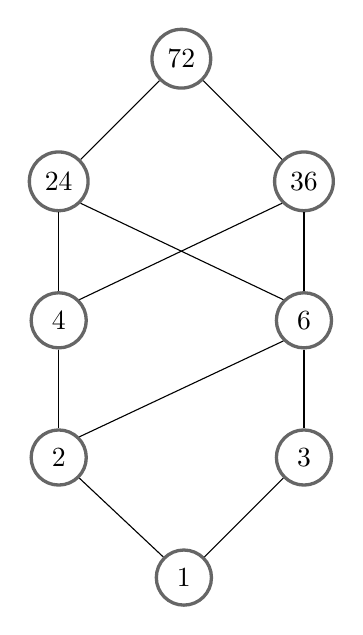
\begin{tikzpicture}[
			roundnode/.style={circle, draw=black!60, very thick, minimum size=7mm},
			]
			%Nodes
			\node[roundnode]      (toplayer)   {72};
			\node[roundnode]      (1layer1)    [below left=of toplayer] {24};
			\node[roundnode]      (1layer2)    [below right=of toplayer] {36};
			\node[roundnode]      (2layer1)    [below=of 1layer1] {4};
			\node[roundnode]      (2layer2)    [below=of 1layer2] {6};
			\node[roundnode]      (3layer1)    [below=of 2layer1] {2};
			\node[roundnode]      (3layer2)    [below=of 2layer2] {3};
			\node[roundnode]      (bottomlayer)    [below left=of 3layer2] {1};
			
			%Lines
			\draw[-] (toplayer.south west) -- (1layer1.north east);
			\draw[-] (toplayer.south east) -- (1layer2.north west);
			\draw[-] (1layer1.south) -- (2layer1.north);
			\draw[-] (1layer1.south east) -- (2layer2.north west);
			\draw[-] (1layer2.south west) -- (2layer1.north east);
			\draw[-] (1layer2.south) -- (2layer2.north);
			\draw[-] (2layer1.south) -- (3layer1.north);
			\draw[-] (2layer2.south west) -- (3layer1.north east);
			\draw[-] (2layer2.south) -- (3layer2.north);
			\draw[-] (3layer1.south east) -- (bottomlayer.north west);
			\draw[-] (3layer2.south west) -- (bottomlayer.north east);
		\end{tikzpicture}
	}
	\hspace{.15\linewidth}
	\resizebox{.3\linewidth}{15em}{
		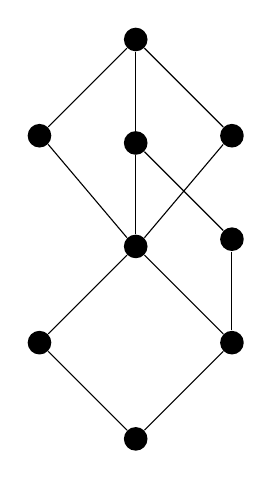
\begin{tikzpicture}[
			dotnode/.style={circle, minimum size=3mm, fill=black, node font=\tiny},
			]
			%Nodes
			\node[dotnode]      (toplayer) {};
			\node[dotnode]      (1layer1)    [below left=of toplayer] {};
			\node[dotnode]      (1layer2)    [below=of toplayer] {};
			\node[dotnode]      (1layer3)    [below right=of toplayer] {};
			\node[dotnode]      (2layer1)    [below=of 1layer2] {};
			\node[dotnode]      (2layer2)    [below=of 1layer3] {};
			\node[dotnode]      (3layer1)    [below left=of 2layer1] {};
			\node[dotnode]      (3layer2)    [below=of 2layer2] {};
			\node[dotnode]      (bottomlayer)    [below left=of 3layer2] {};
			
			%Lines
			\draw[-] (toplayer.south west) -- (1layer1.north east);
			\draw[-] (toplayer.south) -- (1layer2.north);
			\draw[-] (toplayer.south east) -- (1layer3.north west);
			\draw[-] (1layer1.south east) -- (2layer1.north west);
			\draw[-] (1layer2.south) -- (2layer1.north);
			\draw[-] (1layer2.south east) -- (2layer2.north west);
			\draw[-] (1layer3.south west) -- (2layer1.north east);
			\draw[-] (2layer1.south west) -- (3layer1.north east);
			\draw[-] (2layer1.south east) -- (3layer2.north west);
			\draw[-] (2layer2.south) -- (3layer2.north);
			\draw[-] (3layer1.south east) -- (bottomlayer.north west);
			\draw[-] (3layer2.south west) -- (bottomlayer.north east);
		\end{tikzpicture}
	}
	\end{center}
	
	\begin{definition}
		A lattice elements of which satisfy equations
		\begin{align*}
			x \land (y \lor z) = (x \land y) \lor (x \land z),\\
			x \lor (y \land z) = (x \lor y) \land (x \lor z)
		\end{align*}
		is called \textit{distributive}.
	\end{definition}
	
	\begin{theorem} 
		A lattice is distributive iff it contains (a sublattice which is) neither a pentagon, nor a diamond.
	\end{theorem}
	
	\begin{definition}
		A lattice such that if $x\leq z$, then $x\lor (y \land z) = (x \lor y) \land z$ is called \textit{modular}.
	\end{definition}
	
	\begin{theorem} 
		A lattice is modular iff it does not contain (a sublattice which is) a pentagon.
	\end{theorem}
	
	\noindent\textbf{Solution.} Let us consider the first diagram. It represents poset
	\[(\{1,\,2,\,3,\,4,\,5,\,6,\,24,\,36,\,72\},|).\]
	First, we have to find out whether this diagram indeed represents a lattice by finding suprema and infima of all pairs of incomparable elements.
	\begin{itemize}
		\item $24 \land 36$ does not exist, $4 \land 6 = 2$, $2 \land 3 = 1$;
		\item $24 \lor 36 = 72$, $4 \lor 6$ does not exist, $2 \lor 3 = 6$.
	\end{itemize}
	Since there is a pair of elements which does not have infimum and a pair which does not have supremum, this object cannot be considered lattice, therefore distributivity and modularity do not apply to the object represented by the first diagram.
	
	Let us consider the second diagram. For the sake of clarity, we will assign a one-letter name for each node while naming top and bottom nodes 0 and 1 respectively. Resulting diagram:
	\begin{center}
		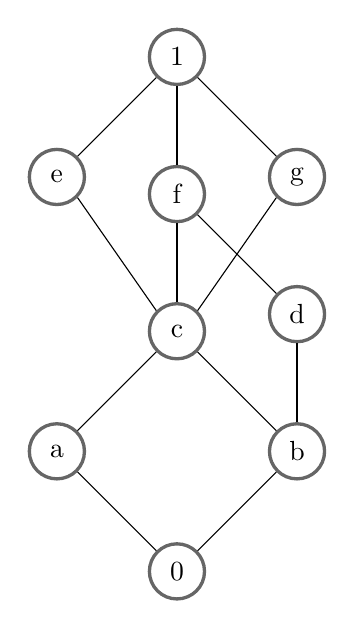
\begin{tikzpicture}[
			roundnode/.style={circle, draw=black!60, very thick, minimum size=7mm},
			]
			%Nodes
			\node[roundnode]      (toplayer) {1};
			\node[roundnode]      (1layer1)    [below left=of toplayer] {e};
			\node[roundnode]      (1layer2)    [below=of toplayer] {f};
			\node[roundnode]      (1layer3)    [below right=of toplayer] {g};
			\node[roundnode]      (2layer1)    [below=of 1layer2] {c};
			\node[roundnode]      (2layer2)    [below=of 1layer3] {d};
			\node[roundnode]      (3layer1)    [below left=of 2layer1] {a};
			\node[roundnode]      (3layer2)    [below=of 2layer2] {b};
			\node[roundnode]      (bottomlayer)    [below left=of 3layer2] {0};
			
			%Lines
			\draw[-] (toplayer.south west) -- (1layer1.north east);
			\draw[-] (toplayer.south) -- (1layer2.north);
			\draw[-] (toplayer.south east) -- (1layer3.north west);
			\draw[-] (1layer1.south east) -- (2layer1.north west);
			\draw[-] (1layer2.south) -- (2layer1.north);
			\draw[-] (1layer2.south east) -- (2layer2.north west);
			\draw[-] (1layer3.south west) -- (2layer1.north east);
			\draw[-] (2layer1.south west) -- (3layer1.north east);
			\draw[-] (2layer1.south east) -- (3layer2.north west);
			\draw[-] (2layer2.south) -- (3layer2.north);
			\draw[-] (3layer1.south east) -- (bottomlayer.north west);
			\draw[-] (3layer2.south west) -- (bottomlayer.north east);
		\end{tikzpicture}
	\end{center}
	Again, we have to check whether this diagram represents a lattice. 
	\begin{itemize}
		\item \textit{Infima.} $a \land b = 0$, $c \land d = b$, $e \land f = c$, $e \land g = c$, $f \land g = c$.
		\item \textit{Suprema.} $a \lor b = c$, $c \lor d = f$, $e \lor f = 1$, $e \lor g = 1$, $f \lor g = 1$.
	\end{itemize}
	Since each pair of incomparable elements has infinum and supremum, the diagram represents a lattice. 
	
	This diagram contains a sublattice $\{c,\, e,\, f,\, g,\, 1\}$ which is a diamond. Therefore, according to Theorem 1, it cannot be distributive. However, this diagram does not contain any pentagons, hence, according to Theorem 2, it is modular.
	
	\newpage
	\subsection*{Question 4}
	
	\noindent\textbf{Task.}  Show that distributivity implies absorption.
	
	\noindent\textbf{Solution.} 
	
	\newpage
	\subsection*{Question 5}
	
	\noindent\textbf{Task.}  Prove the following two rules using only Armstrong rules without using the properties of the operation $(\cdot)^\prime$.
	\begin{enumerate}
		\item $\dfrac{X\rightarrow Y\cup Z}{X\rightarrow Y; X\rightarrow Z}$,
		\item $\dfrac{X \rightarrow Y\setminus X}{X \rightarrow Y}$.
	\end{enumerate}
	\noindent\textbf{Solution.} 
	\begin{enumerate}
		\item Using second Armstrong rule twice we get at first $\dfrac{Y\rightarrow Y}{Y\cup Z\rightarrow Y}$ and then $\dfrac{Y\cup Z\rightarrow Y}{(Y\cup Z) \cup X\rightarrow Y}$. After that, using third Armstrong rule we get 
		\[\dfrac{X\rightarrow Y\cup Z,\, (Y \cup Z) \cup X \rightarrow Y}{X\rightarrow Y},\]
		dually, after applying second Armstrong rule twice and third Armstrong rule once we get $\dfrac{X\rightarrow Y\cup Z,\, (Z \cup Y) \cup X \rightarrow Z}{X\rightarrow Z}$; QED.
		\item $\dfrac{X \rightarrow Y\setminus X}{X \rightarrow Y}$. Let $Y=X\cup X_1$. Using first Armstrong rule, we get $\dfrac{}{X_1\cup X\rightarrow X\cup X_1}$, then using third rule we get 
		\[\dfrac{X\rightarrow X_1,\, X_1\cup X\rightarrow X\cup X_1}{X\rightarrow X\cup X_1}; \text{QED}.\]
	\end{enumerate}
\end{document}